\section{Problem Statement and DR Background}
\label{sec:background}

We provide background on dimensionality reduction (DR) and revisit a widely cited empirical comparison of DR techniques from VLDB 2008~\cite{keogh-study} \red{that we use as a case study.
We show} that Principal Component Analysis (PCA) can outperform classic techniques, but at a high computational cost.

\subsection{Dimensionality Reduction}
\label{sec:defs}

%As time series grow larger and richer with respect to the number of metrics and metadata collected (e.g., as sensor fidelity and sampling rates increase), DR becomes important in their analysis~\cite{macrobase}.
DR refers to finding a low-dimensional representation of a dataset that preserves properties of interest, such as data point similarity~\cite{dr-survey1,dr-survey2}.
Formally, consider $\mvar$ data vectors of length $\dvar$, $x_i \in \mathbb{R}^\dvar$, with $\mvar > \dvar$. 
We can represent this as a dataset matrix $X \in \mathbb{R}^{\mvar \times \dvar}$, where each row $i$ corresponds to vector $x_i$.  
DR computes a transformation function ($T: \mathbb{R}^\dvar \rightarrow \mathbb{R}^k$) that maps each $x_i$ to a new basis as $\tilde{x}_i \in \mathbb{R}^k$ where $k \leq \dvar$, resulting in a new data matrix $T(X) = \tilde{X} \in \mathbb{R}^{\mvar \times k}$ that preserves some metric of interest.  

DR techniques optimize for various metrics. 
%For instance, DR via Locality Sensitive Hashing~\cite{lsh} can preserve distance metrics such as Hamming distance and Jaccard similarity, and
In similarity search, for instance, a popular metric to preserve is the average Euclidean distance between pairs of points, which the literature refers to as \emph{tightness of lower bounds} ($TLB$)~\cite{gemini,keogh-study}.


\subsubsection*{Principal Component Analysis (PCA)}
\label{sec:pca}
PCA is a linear DR technique that identifies a new orthogonal basis for a dataset that captures its directions of highest variance.
Of all linear transformations, this basis minimizes reconstruction error in a mean square sense. 
Classically implemented PCA uses a Singular Value Decomposition (SVD) routine~\cite{trefethen}.
%, which computes the matrix decomposition $X = U \Sigma V^\intercal$.  
%Given a data matrix $X$, PCA via SVD forms the PCA transformation matrix $T:\mathbb{R}^\dvar \rightarrow \mathbb{R}^k$ by first subtracting each column in $X$ by the column's mean to obtain $C_X$ ($\mathbf{1}^\intercal C_X = \mathbf{0}$). 
%The first $k$ right singular vectors of $C_X$ (first $k$ columns of $V$ from the SVD of $C_X$) comprise $T$.  

\begin{comment} 
\begin{algorithm}
\begin{algorithmic}[1]
\Statex \textbf{Inputs:}  
\Statex $X \in \mathbb{R}^{m_1 \times d}$: training data matrix 
\Statex $Y \in \mathbb{R}^{m_2 \times d}$: data matrix to transform 
\Statex $k \in \mathbb{Z}_+$: desired dimensionality of transformed data
\Statex \textsc{SVD-T}: any truncated SVD algorithm  
\Statex
\Statex \hrule
\Function{fit}{$X$}:
	\State $\bar{X} = \text{columnMeans}(X)$
	\State $C_X = X - \bar{X}$
		\Comment{$C_X \in \mathbb{R}^{m_1 \times d}$}
	\State \textbf{Store: } $\bar{X}, C_A$
\EndFunction

\Function{transform}{$Y, k, $ \textsc{SVD-T}}:
	\State $U, \Sigma, V^T$ = \textsc{SVD-T}$(C_X, k)$
		\Comment{$V \in \mathbb{R}^{d \times k}$}
	\State $C_Y = Y - \bar{X}$
		\Comment{$C_Y \in \mathbb{R}^{m_2 \times d}$} 
	\State \textbf{Store: } $T = V$ 
			\Comment{Cache for repeated use} \\
	\Return $C_YT$
		%\Comment{$C_BV \in \mathbb{R}^{M_2 \times k}$} 
\EndFunction

\end{algorithmic}
\caption{PCA via truncated SVD}
\label{alg:PCA-inc}
\end{algorithm}

%discuss advanced techniques
As described in Section~\ref{related}, several theoretical advances provide accelerated means of of efficiently computing PCA over large-scale data beyond the na\"ive SVD-based approach.
These methods operate on samples of input data, and---in theory---confer substantial runtime benefits when in fact a low-dimensional basis exists (i.e., the spectrum of eigenvalues has a large drop).
However, there are two main challenges in utilizing these approaches.
First, it is unclear when to stop sampling data points when using stochastic or mini-batch methods, including state-of-the-art momentum techniques that achieve accelerated convergence rates~\cite{CDS}.
This is because convergence of these techniques (e.g., the magnitude of the gradient in stochastic gradient methods) does not correspond directly to preservation of metrics of interest.
Second, these techniques typically rely the target reduced dimension ($k$) to be specified a priori, but the suitable $k$ for the task at hand is rarely known a priori for a given dataset. The choice of $k$ can dramatically affect runtimes and convergence rates, making the target dimensionality an important, yet difficult to obtain parameter. 

Thus, even with advanced techniques, it is unclear \emph{how much computation is required} to obtain acceptable low dimensional representations, and \emph{how low a dimension is considered acceptable} for specific application constraints. 
We describe how DROP overcomes these challenges in [forward ref sampling], and show how answering these questions enables improvements over previous techniques when evaluated in an end-to-end context.  
\end{comment}

\subsection{DR \red{for Repeated-Query Workloads}}

In workloads such as similarity search, clustering, \red{or classification}, ML models are periodically trained over historical data, and are \emph{repeatedly queried} as incoming data arrives or new query needs arise (see Fig~\ref{fig:pipeline}). 
Indexes built over this data can improve the efficiency of this repeated query workload in exchange for a preprocessing overhead.
DR with a multidimensional index structure is a classic way of achieving this, and is the basis for popular similarity search procedures and extensions in the data mining and machine learning communities~\cite{keogh-indexing,local-dr,charu-ss,dynamic-ss,dm-book,humming-index,decade,search}; a metric-preserving transformation reduces input dimensionality, and an index is built in this new space for subsequent queries.


\subsubsection*{\red{DR in Similarity Search}}
\red{Similarity search is a common repeated-query workload performed over a variety of data types including images, documents and time series~\cite{keogh-study,lsh}, which we use as a running case study.
The $TLB$ is useful here to identify the quality of a low dimensional transformation without performing the downstream similarity search task, as it measures how well a \emph{contractive} DR transformation (i.e. distances in the transformed space are less than or equal to those in the original) preserves pairwise Euclidean distances:}
\begin{equation}
\label{eq:tlb}
TLB = \frac{2}{\mvar(\mvar-1)}\sum_{i<j}\frac{\| \tilde{x}_i -  \tilde{x}_j \|_2 }{\| x_i -  x_j\|_2 }.
\end{equation}
%If $TLB$ is preserved (close to 1), then nearby points remain nearby and far away points remain far away. 
We focus on Euclidean time series similarity search \red{as our primary means of evaluation} given its popularity and the large amount of research in the space.%; we discuss alternatives in Sections~\ref{subsec:teval}.% and~\ref{subsec:disc}.

%By performing DR as a data pre-processing step, downstream analytics operators for tasks including clustering, classification, and similarity search can operate over substantially smaller data. 
%As an example, Figure~\ref{fig:plain_knn} demonstrates how K-Nearest Neighbor (k-NN) runtime scales with dataset size ($m$) and dimensionality ($n$) using the experimental setup described in Section~\ref{sec:experiments}.
%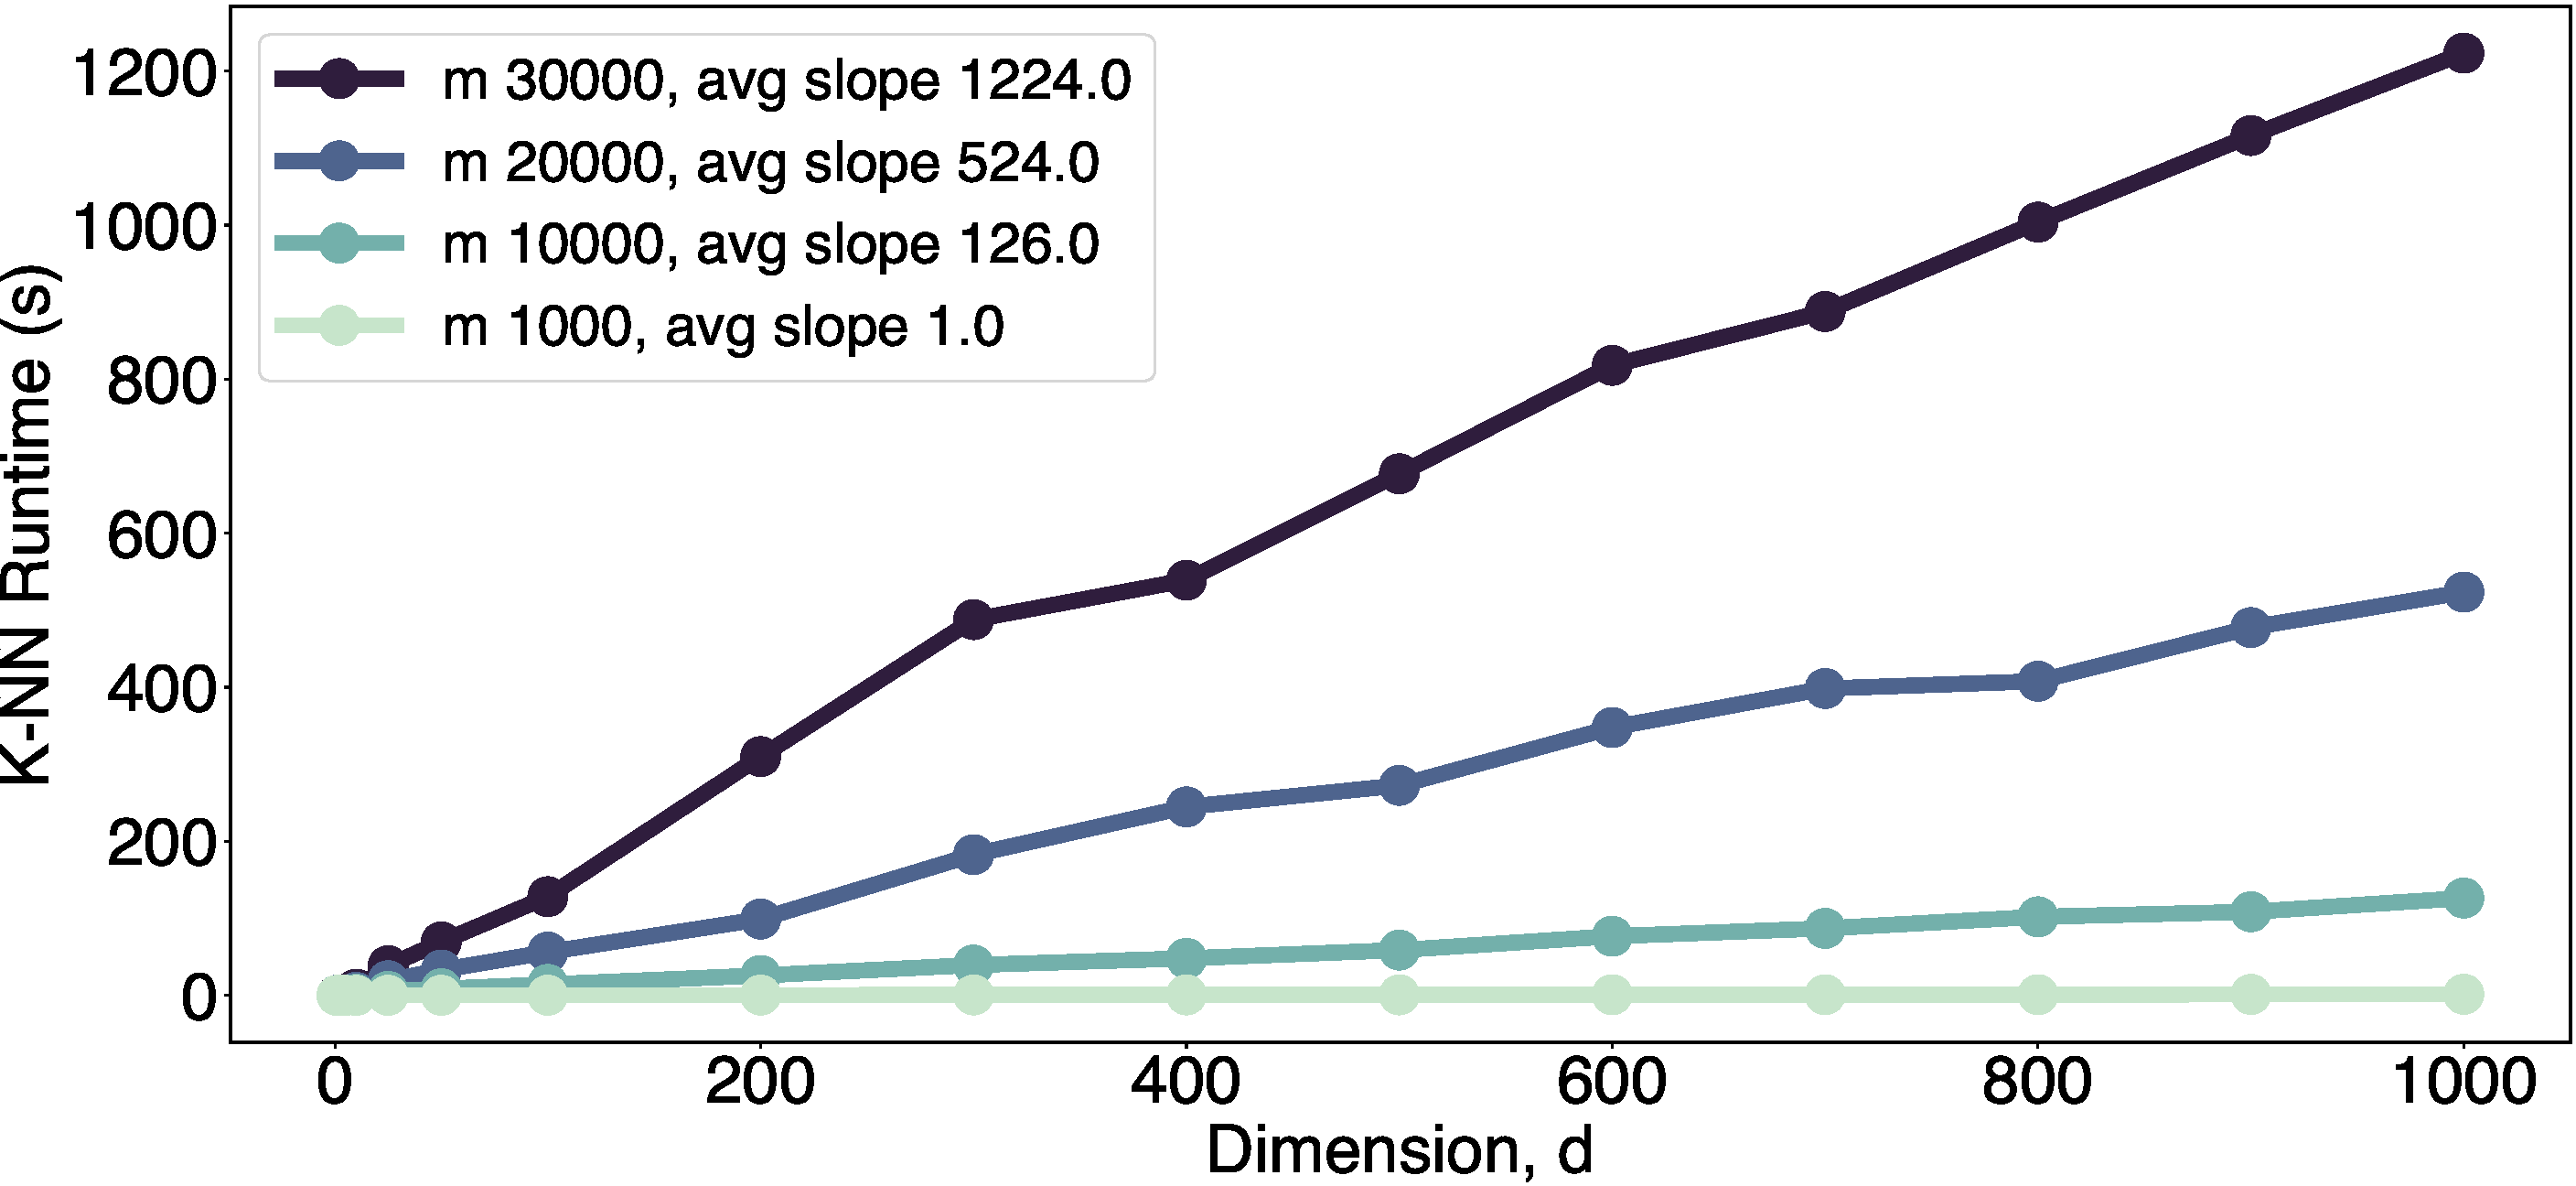
\includegraphics[width=.9\linewidth]{figs/knn_runtime_scaling.pdf}
%We see that the smaller the data dimensionality, the lower the runtime cost---and \emph{larger datasets see greater improvements} as dimensionality is decreased.

%\begin{figure}
%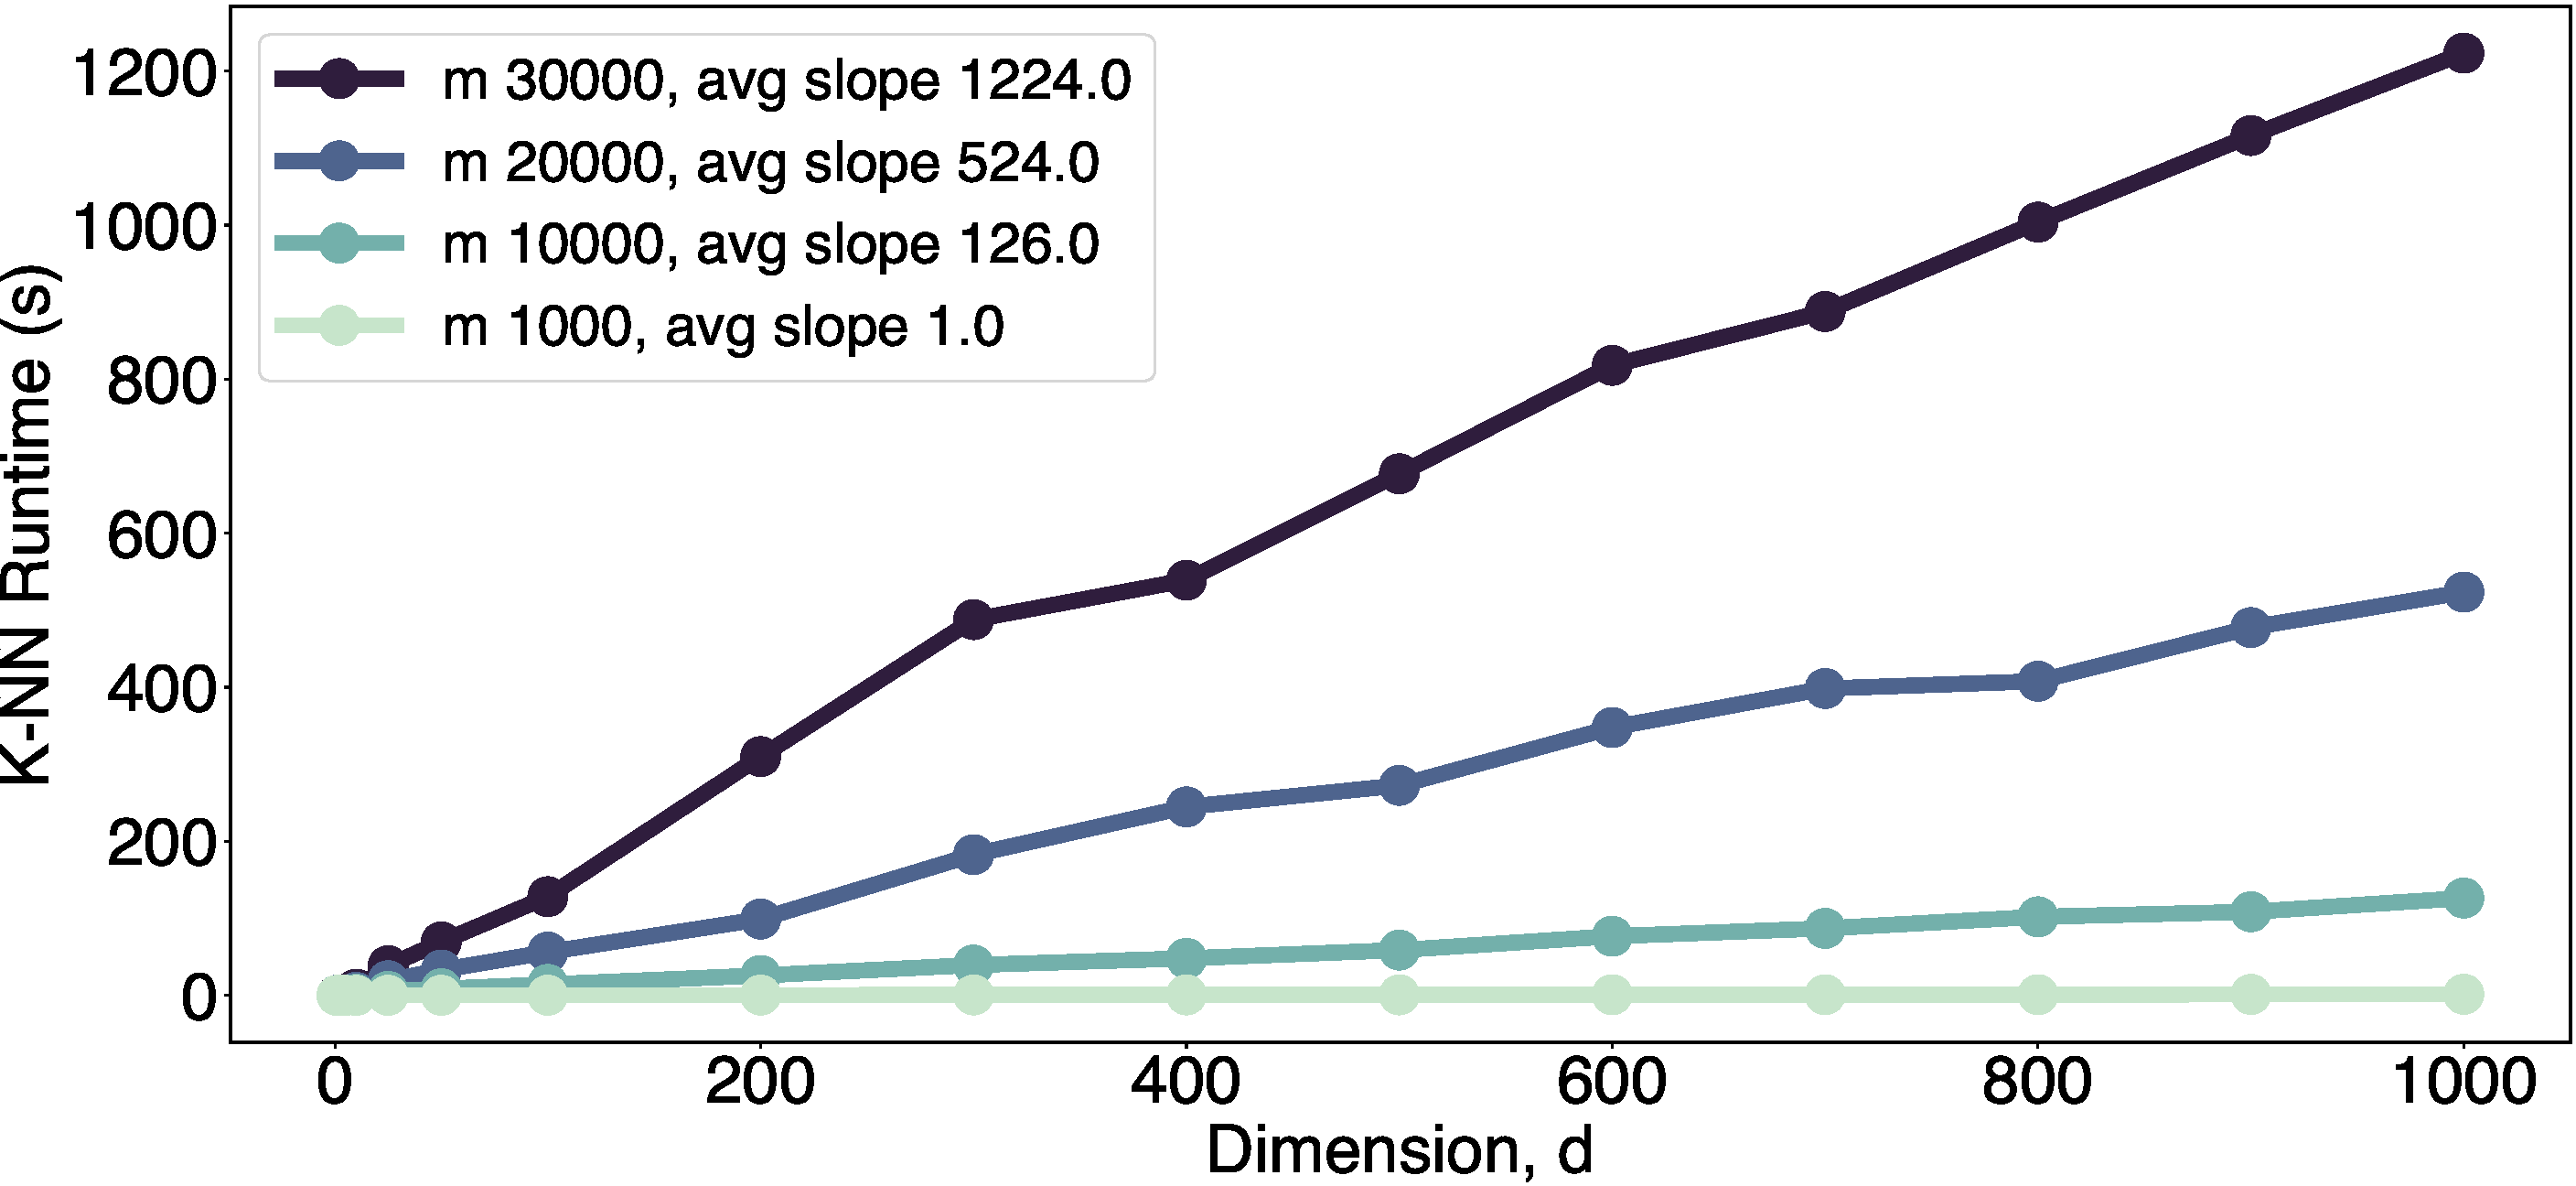
\includegraphics[width=\linewidth]{figs/knn_runtime_scaling.pdf}
%\caption[]{Runtime of k-NN (specifically, 1-NN) as data dimensionality varies. For a given dataset size ($m$) operating with lower dimensionality ($d$) provides linear runtime improvements. This improvement grows as dataset size grows.}
%\label{fig:plain_knn}
%\end{figure}


\subsection{Case Study: PCA Speed vs. Quality}

While improved quality provides faster repeated query execution (as seen in Section~\ref{sec:experiments}), the cost of DR via PCA dominates this speedup, encouraging the use of faster, lower-quality alternatives~\cite{keogh-study}. 
This motivates our study of downstream-workload-aware, stochastic, sampling-based PCA methods.

To briefly quantify this trade-off, we augment a widely-cited time series similarity search DR study from VLDB 2008~\cite{keogh-study} by evaluating PCA---which the authors did not benchmark due to it being ``untenable for large data sets" despite providing ``optimal linear dimensionality reduction."
We compare PCA via SVD to baseline techniques based on both runtime and DR performance with respect to $TLB$ over the largest datasets from~\cite{keogh-study}. 
We use two of their fastest methods as our baselines since they show the remainder exhibited ``very little difference'': Fast Fourier Transform (FFT) and Piecewise Aggregate Approximation (PAA).
We verify that PCA offers more effective dimensionality reduction than alternative techniques for time series similarity search, but with a large computational overhead. 


\minihead{TLB Performance Comparison}
We compute the minimum dimensionality ($k$) achieved by each technique subject to a $TLB$ constraint. 
On average across the datasets, PCA provides bases that are $2.3\times$ and $3.7\times$  smaller than PAA and FFT for $TLB = 0.75$, and $2.9\times$ and $1.8\times$ smaller for $TLB = 0.99$.
While the margin between PCA and alternatives is dataset-dependent, PCA almost always preserves $TLB$ with a lower dimensional representation.

%\section{Additional End-to-End Plots}
%\input{endendplots}

\minihead{Runtime Performance Comparison} 
PCA implemented via out-of-the-box SVD is on average over \red{$26\times$ (up to $56\times$)} slower than PAA and over \red{$4.6\times$ (up to $9.7\times$)} times slower than FFT when computing the smallest $TLB$-preserving basis.
This substantiates the observation that classic PCA is incredibly slow compared to alternatives~\cite{keogh-study}. 


